\nonstopmode
\documentclass[10pt,letterpaper]{article}

% --- Page geometry ---
\usepackage[top=1in,bottom=1in,left=0.75in,right=0.75in,
            columnsep=0.25in]{geometry}

% --- Core packages ---
\usepackage{amsmath,amssymb}
\usepackage{graphicx}
\graphicspath{{./}{.}}
\usepackage{booktabs}
\usepackage{multirow}
\usepackage[colorlinks=true,urlcolor=blue,citecolor=blue,
            linkcolor=blue]{hyperref}
\usepackage{microtype}         % microtypography — fixes 90% of line-break issues
\usepackage{xurl}              % allows URL line breaks anywhere
\usepackage[all]{hypcap}       % fix hyperref anchors: links jump to top of float, not caption
\usepackage{float}             % provides [H] specifier: place float exactly here
\setlength{\abovecaptionskip}{2pt}  % reduce space above captions in tables/figures
\setlength{\belowcaptionskip}{2pt}  % reduce space below captions

% --- Typography ---
\emergencystretch=3em          % prevents remaining underfull hboxes

% --- Section formatting (PRL-style) ---
\usepackage{titlesec}
\titleformat{\section}
  {\normalsize\bfseries\centering}{}{0pt}
  {\MakeUppercase}
\titleformat{\subsection}
  {\normalsize\itshape}{}{0pt}{}
\titlespacing{\section}{0pt}{6pt plus 2pt minus 2pt}{3pt}
\titlespacing{\subsection}{0pt}{4pt plus 1pt}{2pt}

\setlength{\parindent}{1em}
\setlength{\parskip}{2pt plus 1pt}
\usepackage{url}
\def\UrlBreaks{\do\/\do-\do.\do\_}
\def\UrlNoBreaks{\do\:}
% ============================================================
\begin{document}

% --- Title block (full-width, above two-column body) ---
\twocolumn[{%
  \centering
  {\large\bfseries Fluid-Dynamic Stability Filtering for Zero-Noise
    Extrapolation in NISQ-Era Quantum Circuits}\\[6pt]
  {\normalsize Shawn G. Kleipe}\\[2pt]
  {\small\itshape Independent Researcher,
    \href{https://orcid.org/0009-0002-2480-2430}%
         {ORCID: 0009-0002-2480-2430}}\\[2pt]
  {\small v0.4.0 --- \today}\\[8pt]

  \begin{minipage}{0.92\textwidth}\small
  \textbf{Abstract.}
  Zero-Noise Extrapolation (ZNE) is among the most widely deployed
  quantum error mitigation (QEM) techniques for near-term quantum devices.
  However, the choice of noise scaling schedule remains largely empirical,
  and no standard method exists for validating whether a given ZNE
  extrapolation is physically reliable or has diverged into an artifact.
  We introduce two contributions: (i)~a fluid-dynamic stability filter
  motivated by the structure of the Navier-Stokes energy dissipation norm,
  defining $\varepsilon = \nu\int_{\Omega}\|\nabla\mathbf{u}\|^{2}\,d\Omega$
  and flagging a ZNE output as unreliable when $\varepsilon \geq \Gamma$,
  as a post-hoc reliability criterion; (ii)~a family of structured noise
  scaling schedules --- Fibonacci ($\tau_{n}=\tau_{n-1}+\tau_{n-2}$),
  Lucas, and prime-anchored --- as alternatives to conventional linear
  or odd-integer scaling, evaluated against all four standard extrapolants
  (linear, Richardson, poly-2, poly-3).
  We evaluate both across circuit depths $d\in\{2,4,6,8,10,12,16,20\}$,
  depolarizing noise levels
  $p\in\{0.001,0.005,0.01,0.02,0.05,0.1,0.15,0.2\}$, and qubit counts
  $n\in\{2,4,6\}$ using shot-based density matrix simulation in Cirq,
  totalling 153,600 experiment runs
  (4 circuit types $\times$ 5 schedules $\times$ 4 extrapolants
  $\times$ 3 qubit counts $\times$ 8 depths $\times$ 8 noise levels
  $\times$ 10 trials).
  The stability filter achieves 0 flags in 14,400 independent trials
  (1,440 configurations $\times$ 10 trials) at $p\leq 0.01$,
  $d\leq 4$, giving a 95\% Clopper-Pearson upper bound of
  $p_{\mathrm{flag}}<0.00022$ across all configurations.
  Mean $\varepsilon$ follows the ordering
  VQE (mean $0.020$) $>$ QAOA (mean $0.017$) $>$
  random (mean $0.012$) $>$ test (mean $0.008$)
  (ranges: $0.014$--$0.024$, $0.012$--$0.022$, $0.010$--$0.016$,
  $0.004$--$0.013$ respectively; ordering holds schedule-by-schedule
  across all five, at the reference condition),
  a previously uncharacterised dependence now extended to QAOA and
  three qubit counts.
  The energy norm $\varepsilon$ decreases monotonically with qubit count
  in 19 of 20 circuit/schedule combinations.
  Across all four extrapolants, linear extrapolation produces the lowest
  and most consistent ZNE variance; Lucas achieves the lowest variance
  on random and QAOA circuits.
  Hardware validation on ibm\_fez (Heron~r2) and ibm\_torino (Heron~r1)
  confirms zero flags in 120 independent trials (24 conditions
  $\times$ 5 trials) across all four circuit types and
  $d\in\{2,4,6,8\}$, with maximum observed
  $\varepsilon=0.00285$ ($5.7\%$ of $\Gamma$).
  Code is available at GitHub and archived at Zenodo.\\[4pt]
  \textit{PACS: 03.67.Pp, 03.67.Lx, 47.10.ad}
  \end{minipage}
  \vspace{10pt}\par
}]

% ============================================================
\section{Introduction}
% ============================================================

Quantum computing devices in the noisy intermediate-scale quantum
(NISQ) era~\cite{Preskill2018} are fundamentally limited by decoherence
and gate errors. Quantum Error Mitigation (QEM) aims to extract
near-noiseless expectation values from noisy circuits without the qubit
overhead of full error correction~\cite{Temme2017,Endo2018}.

Zero-Noise Extrapolation (ZNE)~\cite{Temme2017,Li2017} is the most
widely adopted QEM method, implemented in tools such as
Mitiq~\cite{LaRose2022}. Despite widespread use, two fundamental
questions remain open: (1)~\textit{Schedule selection} --- linear scale
factors $\lambda\in\{1,2,3,\ldots\}$ are the de facto standard but their
optimality is unestablished; (2)~\textit{Reliability validation} --- no
standard criterion distinguishes physically meaningful ZNE outputs from
extrapolation artifacts (``hallucinations'').

We address both. For~(1), we propose and compare five noise scaling
schedules: Fibonacci (golden-ratio spacing), Lucas, and prime-anchored
sequences as novel alternatives to the conventional linear and
odd-integer schedules, and evaluate all five against four extrapolants
(linear, Richardson, poly-2, poly-3) across four circuit types including
QAOA. For~(2), we introduce a stability criterion inspired by
fluid-dynamic energy dissipation theory.
Both contributions are validated on IBM Quantum hardware
(ibm\_fez and ibm\_torino) in addition to simulation.

% ============================================================
\section{Related Work}
% ============================================================

\subsection{ZNE Variants}
Since its introduction by Temme et al.~\cite{Temme2017} and Li and
Benjamin~\cite{Li2017}, ZNE has been extended in several directions.
Temme et al.~\cite{Temme2017} also introduced Probabilistic Error
Cancellation (PEC) as an alternative QEM strategy; unlike ZNE, PEC
requires a full noise characterisation and incurs exponential sampling
overhead, making ZNE the preferred method when noise is poorly
characterised or sampling budget is limited.
Giurgica-Tiron et al.~\cite{GiurgicaTiron2020} introduced digital noise
scaling via unitary folding and demonstrated error reductions of up to
$24\times$ over non-mitigated circuits.
Krebsbach et al.~\cite{Krebsbach2022} analyzed Richardson extrapolation
specifically for QEM, establishing theoretical bounds on its performance.
Most recently, direct polynomial analysis with explicit error bounds was
provided by~\cite{Mohammadipour2025}, offering the most rigorous
theoretical treatment to date.
Ad hoc reliability checks --- such as comparing poly-2 and poly-3
outputs for consistency, or monitoring extrapolation residuals --- are
used informally in practice but are neither standardised nor
theoretically grounded.
Crucially, none of these works provide a principled post-hoc criterion
for determining whether a specific ZNE output has converged to a
physically meaningful value or diverged into an artifact.
Our stability filter addresses this gap directly.

\subsection{Schedule Selection}
The choice of noise scale factors has received limited formal attention.
Standard implementations use linear~\cite{Temme2017} or
odd-integer~\cite{LaRose2022} schedules, with the latter preferred for
gate-level folding to preserve circuit structure. A noise-aware folding
method~\cite{Hour2024} redistributes noise amplification based on
hardware characteristics, representing the closest prior work to our
schedule investigation. However, no prior work has systematically
compared schedule spacing distributions, proposed golden-ratio-motivated
schedules for ZNE, or evaluated Lucas and prime-anchored sequences as
structured alternatives to conventional integer spacing.

\subsection{ZNE on Hardware}
ZNE has been demonstrated experimentally on superconducting
qubits~\cite{Zhang2025}, silicon spin qubits~\cite{Sohn2025}, and
quantum annealing platforms~\cite{Raymond2025}, confirming its broad
applicability across qubit modalities. Our work validates the
stability filter and schedule comparison on two IBM Quantum processors
(ibm\_fez, Heron~r2; ibm\_torino, Heron~r1), complementary to
these prior hardware demonstrations and extending them to
post-hoc reliability filtering.

\subsection{Physics-Informed Methods}
The use of physical constraints to validate or improve quantum
computations is an emerging direction. Physics-informed neural
networks~\cite{Raissi2019} have been applied to quantum simulation
problems, and stability criteria from fluid dynamics have been used as
convergence monitors in classical numerical methods. To our knowledge,
this is the first work to apply Navier-Stokes energy dissipation norms
as a post-hoc reliability criterion for quantum error mitigation outputs.

% ============================================================
\section{Background}
% ============================================================

\subsection{Zero-Noise Extrapolation}
A noise scale factor $\lambda\geq 1$ produces circuits $\{C_\lambda\}$
with amplified noise. The zero-noise value is estimated by fitting an
extrapolant $f$ to the discrete data and evaluating at $\lambda=0$:
\begin{equation}
  \langle O\rangle_0 \approx
    f\!\left(0;\,\bigl\{(\lambda_k,\langle O\rangle_{\lambda_k})\bigr\}_{k=1}^{K}\right),
\end{equation}
where $f$ is a polynomial or Richardson extrapolant fit to the $K$
measured pairs $\{(\lambda_k,\langle O\rangle_{\lambda_k})\}$.

\subsection{Structured Noise Scaling Sequences}
Fibonacci-based pulse sequences protect against correlated noise in
dynamical decoupling~\cite{Viola1998}, with demonstrated coherence
improvements on superconducting hardware~\cite{Google2023}. We extend
this principle to ZNE noise scale factor selection, and additionally
evaluate the Lucas sequence ($\{2,1,3,4,7,11,\ldots\}$, sorted for
ZNE compatibility: $\{1,2,3,4,7,11\}$) and a prime-anchored sequence, 
both of which share non-uniform, non-harmonic spacing that may reduce 
systematic correlations in noise amplification.

\subsection{Navier-Stokes Energy Dissipation}
The incompressible Navier-Stokes equations are:
\begin{equation}
  \frac{\partial \mathbf{u}}{\partial t}
    + (\mathbf{u}\!\cdot\!\nabla)\mathbf{u}
  = -\nabla P + \nu\nabla^{2}\mathbf{u},\quad
  \nabla\cdot\mathbf{u}=0,
\end{equation}
where $\mathbf{u}$ is the fluid velocity field and $P$ denotes fluid pressure
(distinct from the depolarizing noise
parameter $p$ used throughout the remainder of this paper),
with energy dissipation rate
$\varepsilon = \nu\int_{\Omega}\|\nabla\mathbf{u}\|^{2}\,d\Omega$.
For incompressible flow ($\nabla\cdot\mathbf{u}=0$), integration by
parts shows $2\nu\int_\Omega S_{ij}S_{ij}\,d\Omega =
\nu\int_\Omega\|\nabla\mathbf{u}\|^2\,d\Omega$ (the cross-term
$\int(\partial u_i/\partial x_j)(\partial u_j/\partial x_i)\,d\Omega$
vanishes via $\nabla\cdot\mathbf{u}=0$), so our expression is
equivalent to the standard strain-rate dissipation formulation.
In stable (laminar) flows $\varepsilon$ is bounded; large $\varepsilon$
is associated with strongly unstable or turbulent regimes, and
$\varepsilon$ increases sharply near potential singular
structures~\cite{Tao2016,Wang2025}.

% ============================================================
\section{Method}
% ============================================================

\subsection{Stability Filter}
We identify noise scale factors $\{\lambda_k\}$ with spatial coordinates
and expectation values $\{\langle O\rangle_{\lambda_k}\}$ with velocity.
Under this identification, the velocity gradient $\nabla\mathbf{u}$
corresponds to the slope of the ZNE curve,
$\partial\langle O\rangle/\partial\lambda$, and the squared gradient
norm $\|\nabla\mathbf{u}\|^{2}$ corresponds to
$|\partial\langle O\rangle/\partial\lambda|^{2}$ --- so the
dissipation integral $\nu\int\|\nabla\mathbf{u}\|^{2}\,d\Omega$
maps directly to Eq.~(\ref{eq:eps}) below.
The discrete energy norm is:
\begin{equation}
  \varepsilon \approx \nu\sum_{k}
    \!\left(\frac{\langle O\rangle_{\lambda_{k+1}}
      -\langle O\rangle_{\lambda_k}}
    {\lambda_{k+1}-\lambda_k}\right)^{\!2}\!\Delta\lambda_k,
  \label{eq:eps}
\end{equation}
with $\nu=0.5$, and $\Delta\lambda_k = \lambda_{k+1}-\lambda_k$ is the
scale-factor spacing, so Eq.~(\ref{eq:eps}) is a quadrature
approximation of $\nu\int_{\lambda_1}^{\lambda_K}
|\partial\langle O\rangle/\partial\lambda|^{2}\,d\lambda$ --- a
discrete $H^{1}$ energy seminorm.
A ZNE output is flagged as potentially unreliable
if $\varepsilon\geq\Gamma$ (default $\Gamma=0.05$).
The threshold $\Gamma=0.05$ is chosen to exceed the 99th percentile
of $\varepsilon$ observed under low-noise conditions ($p\leq 0.01$,
$d\leq 4$) by a factor of approximately two (99th percentile: $0.021$;
maximum: $0.024$), providing a conservative margin against shot-noise
fluctuations while remaining sensitive to genuinely unstable regimes.
All quantities in the discrete analog are dimensionless ---
$\lambda_k$ are pure integers, $\langle O\rangle_{\lambda_k}\in[-1,1]$,
and $\nu=0.5$ is a dimensionless constant --- so $\varepsilon$ is a
dimensionless scalar and the threshold comparison $\varepsilon<\Gamma$
is dimensionally consistent.

The identification of noise scale factors with spatial coordinates and
expectation values with a velocity-like field is a \textit{formal analogy},
not a claim that ZNE dynamics are governed by Navier-Stokes equations.
More precisely, $\varepsilon$ is a discrete $H^{1}$ Sobolev
regularity functional on the ZNE curve $\langle O\rangle(\lambda)$:
it measures the \textit{smoothness} of the extrapolation curve rather
than physical energy dissipation.
Smooth ZNE curves ($\varepsilon\ll\Gamma$) correspond to
well-conditioned extrapolation; steep or oscillatory curves
($\varepsilon\geq\Gamma$) indicate sensitivity to noise amplification
and hence unreliable extrapolation.
The connection is a standard condition-number argument: when
$|\partial\langle O\rangle/\partial\lambda|$ is large over the fitting
interval $[\lambda_1,\lambda_K]$, small measurement errors in the
noisy expectation values $\langle O\rangle_{\lambda_k}$ are amplified
by the extrapolation, producing large uncertainty in the zero-noise
estimate $\langle O\rangle_0$.
High $\varepsilon$ directly measures this steepness, making it a
principled proxy for extrapolation ill-conditioning rather than an
empirical heuristic.
The Navier-Stokes norm supplies the mathematical form of the
functional; the interpretation and diagnostic criterion are
defined entirely within the ZNE domain.

\subsection{Hessian Singularity Detection}
As a secondary qualitative consistency check, we examine the Hessian
$H(\Phi)$ of the expectation value surface
$\Phi(\lambda,\theta)$, where $\lambda$ is the noise scale factor and
$\theta$ denotes the circuit parameter vector (e.g.\ rotation angles
for VQE/QAOA circuits; fixed for test and random circuits).
Regions where $\det H < 0$ indicate genuine saddle points (unstable
directions in the landscape); $\det H \approx 0$ indicates degenerate
or ill-conditioned critical points.
This diagnostic is reported as a consistency check alongside the
primary $\varepsilon$-filter, not as an independent quantitative criterion.

\subsection{Fibonacci Noise Scaling Schedule}
\begin{equation}
  \tau_n = \tau_{n-1}+\tau_{n-2},\quad
  \tau_1=1,\;\tau_2=2,
\end{equation}
yielding $\{1,2,3,5,8,13,\ldots\}$, with consecutive terms converging
to $\phi=(1+\sqrt{5})/2\approx 1.618$.
The initial condition $\tau_2=2$ (rather than the conventional
$\tau_2=1$) ensures all $K$ scale factors are distinct, since
$\tau_1=\tau_2=1$ would duplicate the unscaled measurement
$\lambda=1$; our sequence is equivalent to $F_2$ through $F_{K+1}$
in standard Fibonacci indexing.
We additionally evaluate Lucas
($\{1,2,3,4,7,11\}$) and prime-anchored ($\{1,2,3,5,7,11\}$) schedules.

\subsection{Experimental Setup}
All methods use Cirq~\cite{Cirq2023} with Mitiq~\cite{LaRose2022}.

\textit{Observable.} For all $n$-qubit circuits, the measured
observable is the nearest-neighbour correlator on the first pair:
\begin{equation}
  \langle O\rangle = \langle Z_0 Z_1\rangle.
\end{equation}

\textit{Circuit types:} Test (alternating $R_x(\pi/4)$+CNOT); VQE
(hardware-efficient $R_y$+CZ ansatz); Random (randomised single-qubit
gates+CNOT); QAOA (alternating ZZ problem-unitary + $R_x$ mixer).

\textit{Schedules} ($K=6$): Fibonacci $\{1,2,3,5,8,13\}$,
Linear $\{1,2,3,4,5,6\}$, Odd $\{1,3,5,7,9,11\}$,
Lucas $\{1,2,3,4,7,11\}$, Prime-anchored $\{1,2,3,5,7,11\}$.

\textit{Extrapolants:} linear (deg-1), Richardson (two-point),
poly2 (deg-2), poly3 (deg-3).

A single-qubit depolarizing channel with error rate $p$ is applied
independently to each qubit after every gate via
\texttt{cirq.ConstantQubitNoiseModel(\allowbreak cirq.depolarize(p))},
giving an effective two-qubit gate error rate of $1-(1-p)^{2}\approx 2p$,
capped at $p=0.24$ (to keep the effective depolarizing probability
per gate below the regime where density matrix simulation accuracy
degrades significantly; configurations reaching this cap are confined
to the highest noise levels combined with the largest scale factors).
$N=500$ shots, 10 trials;
153,600 total runs ($4\times5\times4\times3\times8\times8\times10$).

% ============================================================
\section{Results}
% ============================================================

All reference results are at $d=4$, $p=0.01$, $K=6$, $N=500$,
10 trials; $n=2$ for Table~\ref{tab:stability}.

\subsection{Stability Filter Performance}

All 1,440 configurations at $p\leq 0.01$, $d\leq 4$ yield zero flags
across all 14,400 trials (95\% Clopper-Pearson upper bound:
$p_{\mathrm{flag}}<0.00022$), confirming the filter is well-calibrated
at moderate depth and noise (Fig.~\ref{fig:heatmap}). At $d\geq 6$ ($p=0.01$) the filter begins flagging
VQE, QAOA, and random circuits; the test circuit first flags at $d=8$
and recurs at $d=16$ (Fig.~\ref{fig:eps_circuits}) --- a period-8
resonance arising from the fixed $R_x(\pi/4)$ rotation schedule, which
drives $\langle Z_0 Z_1\rangle\to\pm 1$ at every eighth layer,
maximising noise sensitivity and ZNE curve steepness.

Mean $\varepsilon$ follows the ordering
VQE (mean $0.020$) $>$ QAOA (mean $0.017$) $>$
random (mean $0.012$) $>$ test (mean $0.008$)
(ranges: $0.014$--$0.024$, $0.012$--$0.022$, $0.010$--$0.016$,
$0.004$--$0.013$ respectively; ordering holds schedule-by-schedule
across all five schedules),
shown in Fig.~\ref{fig:eps_schedules}.
Table~\ref{tab:stability} gives the full $n=2$ reference results.
\begin{table}[H]
\caption{ZNE performance at $d=4$, $p=0.01$, $n=2$, linear extrapolant,
  10 trials. All flag rates 0.0\% ($\Gamma=0.05$).
  std computed with \texttt{ddof=0} (population estimator, $N=10$);
  sample std (\texttt{ddof=1}) is larger by factor
  $\sqrt{N/(N-1)}\approx 1.05$.}
\label{tab:stability}
\centering\small
\setlength{\tabcolsep}{4pt}
\begin{tabular}{llcc}
\toprule
Circuit & Schedule & ZNE (mean $\pm$ std) & $\varepsilon$ \\
\midrule
Test    & Fibonacci & $-0.033\pm 0.022$ & 0.00545 \\
Test    & Linear    & $-0.009\pm 0.044$ & 0.01345 \\
Test    & Odd       & $-0.021\pm 0.031$ & 0.00447 \\
Test    & Lucas     & $-0.022\pm 0.024$ & 0.00801 \\
Test    & Prime     & $-0.016\pm 0.045$ & 0.00757 \\
\midrule
VQE     & Fibonacci & $+0.054\pm 0.324$ & 0.01375 \\
VQE     & Linear    & $-0.025\pm 0.594$ & 0.02408 \\
VQE     & Odd       & $-0.215\pm 0.409$ & 0.01681 \\
VQE     & Lucas     & $-0.085\pm 0.525$ & 0.02318 \\
VQE     & Prime     & $-0.193\pm 0.567$ & 0.01996 \\
\midrule
Random  & Fibonacci & $-0.192\pm 0.275$ & 0.00997 \\
Random  & Linear    & $-0.068\pm 0.447$ & 0.01583 \\
Random  & Odd       & $+0.036\pm 0.441$ & 0.01294 \\
Random  & Lucas     & $-0.002\pm 0.272$ & 0.01023 \\
Random  & Prime     & $+0.081\pm 0.365$ & 0.00956 \\
\midrule
QAOA    & Fibonacci & $+0.001\pm 0.374$ & 0.01249 \\
QAOA    & Linear    & $-0.234\pm 0.547$ & 0.02190 \\
QAOA    & Odd       & $+0.111\pm 0.457$ & 0.01661 \\
QAOA    & Lucas     & $-0.346\pm 0.325$ & 0.01605 \\
QAOA    & Prime     & $+0.209\pm 0.348$ & 0.01727 \\
\bottomrule
\end{tabular}
\end{table}

\subsection{Extrapolant Comparison}

Linear extrapolation consistently produces the lowest variance across
all five schedules (Table~\ref{tab:extrapolants}; Fig.~\ref{fig:extrap_var}). Poly3 is worst in
8 of 20 circuit/schedule combinations; Richardson in 7 of 20.
Richardson is most sensitive on irregular grids (odd, prime-anchored schedules).
Reported standard deviations include a shot-noise contribution of
approximately $0.030$--$0.042$ (estimated from variance propagation
through the OLS intercept for each schedule at $N=500$ shots),
representing $\lesssim 10\%$ of observed $\sigma$ and
$\lesssim 1\%$ of observed variance; schedule rankings and conclusions
are unaffected by this correction.
Linear extrapolation is recommended for reliability-focused deployment.
\begin{table}[H]
\caption{VQE ZNE standard deviation at $d=4$, $p=0.01$, $n=2$.
  Lower std = more consistent.}
\label{tab:extrapolants}
\centering\small
\setlength{\tabcolsep}{5pt}
\begin{tabular}{lcccc}
\toprule
Schedule  & Linear & Richardson & Poly-2 & Poly-3 \\
\midrule
Fibonacci & 0.324  & 0.528      & 0.571  & 0.614  \\
Linear    & 0.594  & 0.424      & 0.523  & 0.650  \\
Odd       & 0.409  & 0.513      & 0.365  & 0.474  \\
Lucas     & 0.525  & 0.342      & 0.529  & 0.347  \\
Prime     & 0.567  & 0.666      & 0.469  & 0.356  \\
\bottomrule
\end{tabular}
\end{table}

\begin{figure*}[tp]
  \centering
  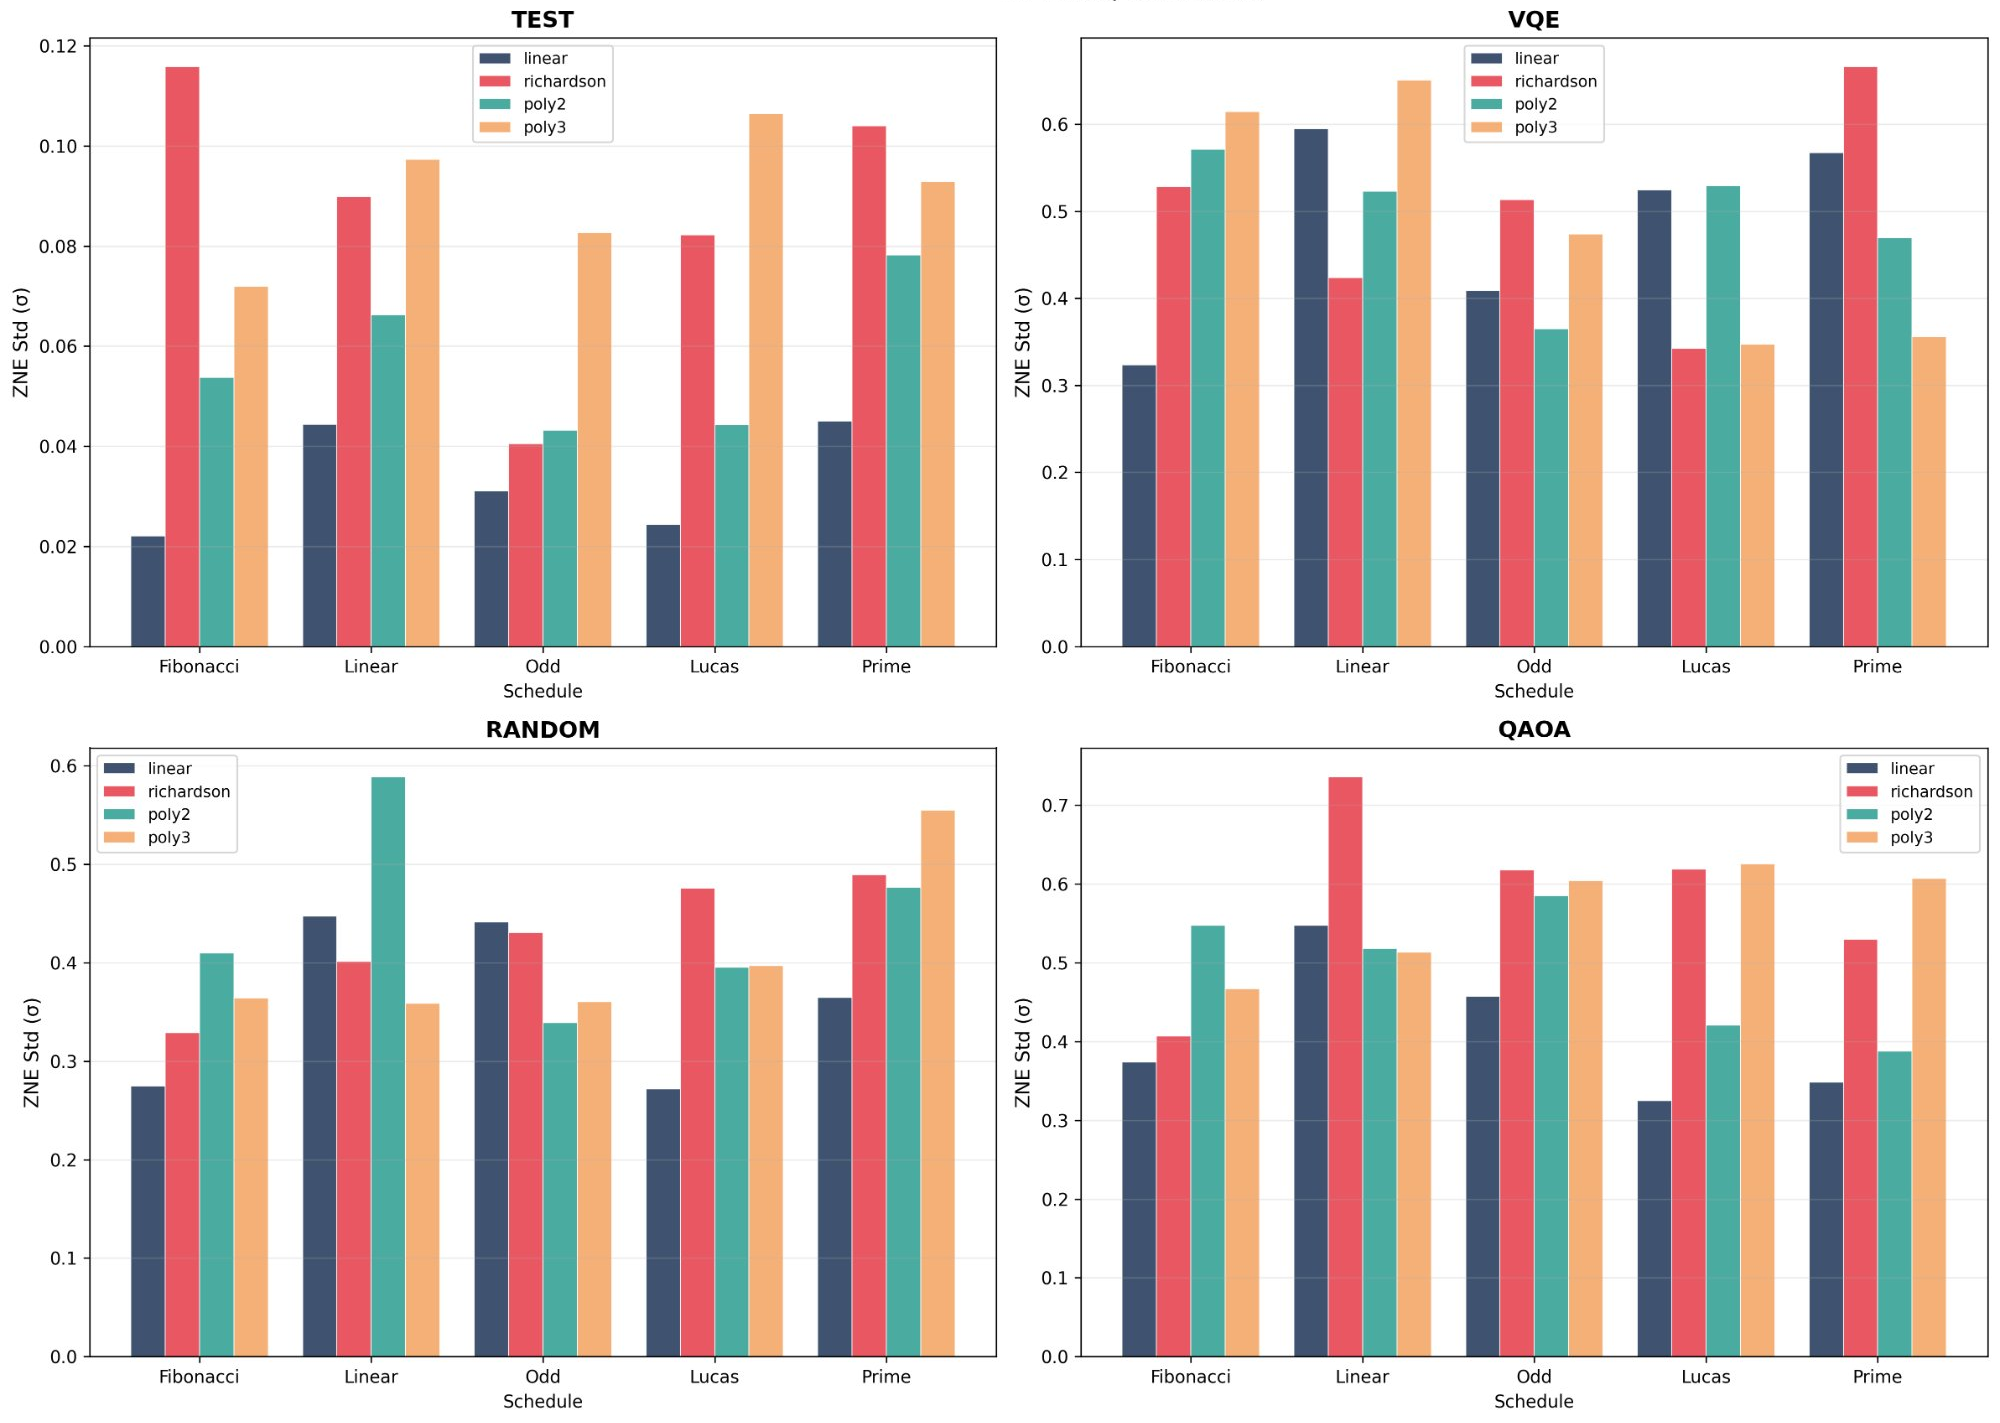
\includegraphics[width=\textwidth]{figD_v4_zne_std_extrapolant_comparison.png}
  \caption{ZNE standard deviation by schedule and extrapolant at
    $d=4$, $p=0.01$, $n=2$, across all four circuit types. Linear
    extrapolation (dark blue) produces the lowest variance for VQE
    across all schedules. Poly-3 and Richardson are worst in
    8/20 and 7/20 circuit/schedule combinations respectively.}
  \label{fig:extrap_var}
\end{figure*}

\begin{figure*}[tp]
  \centering
  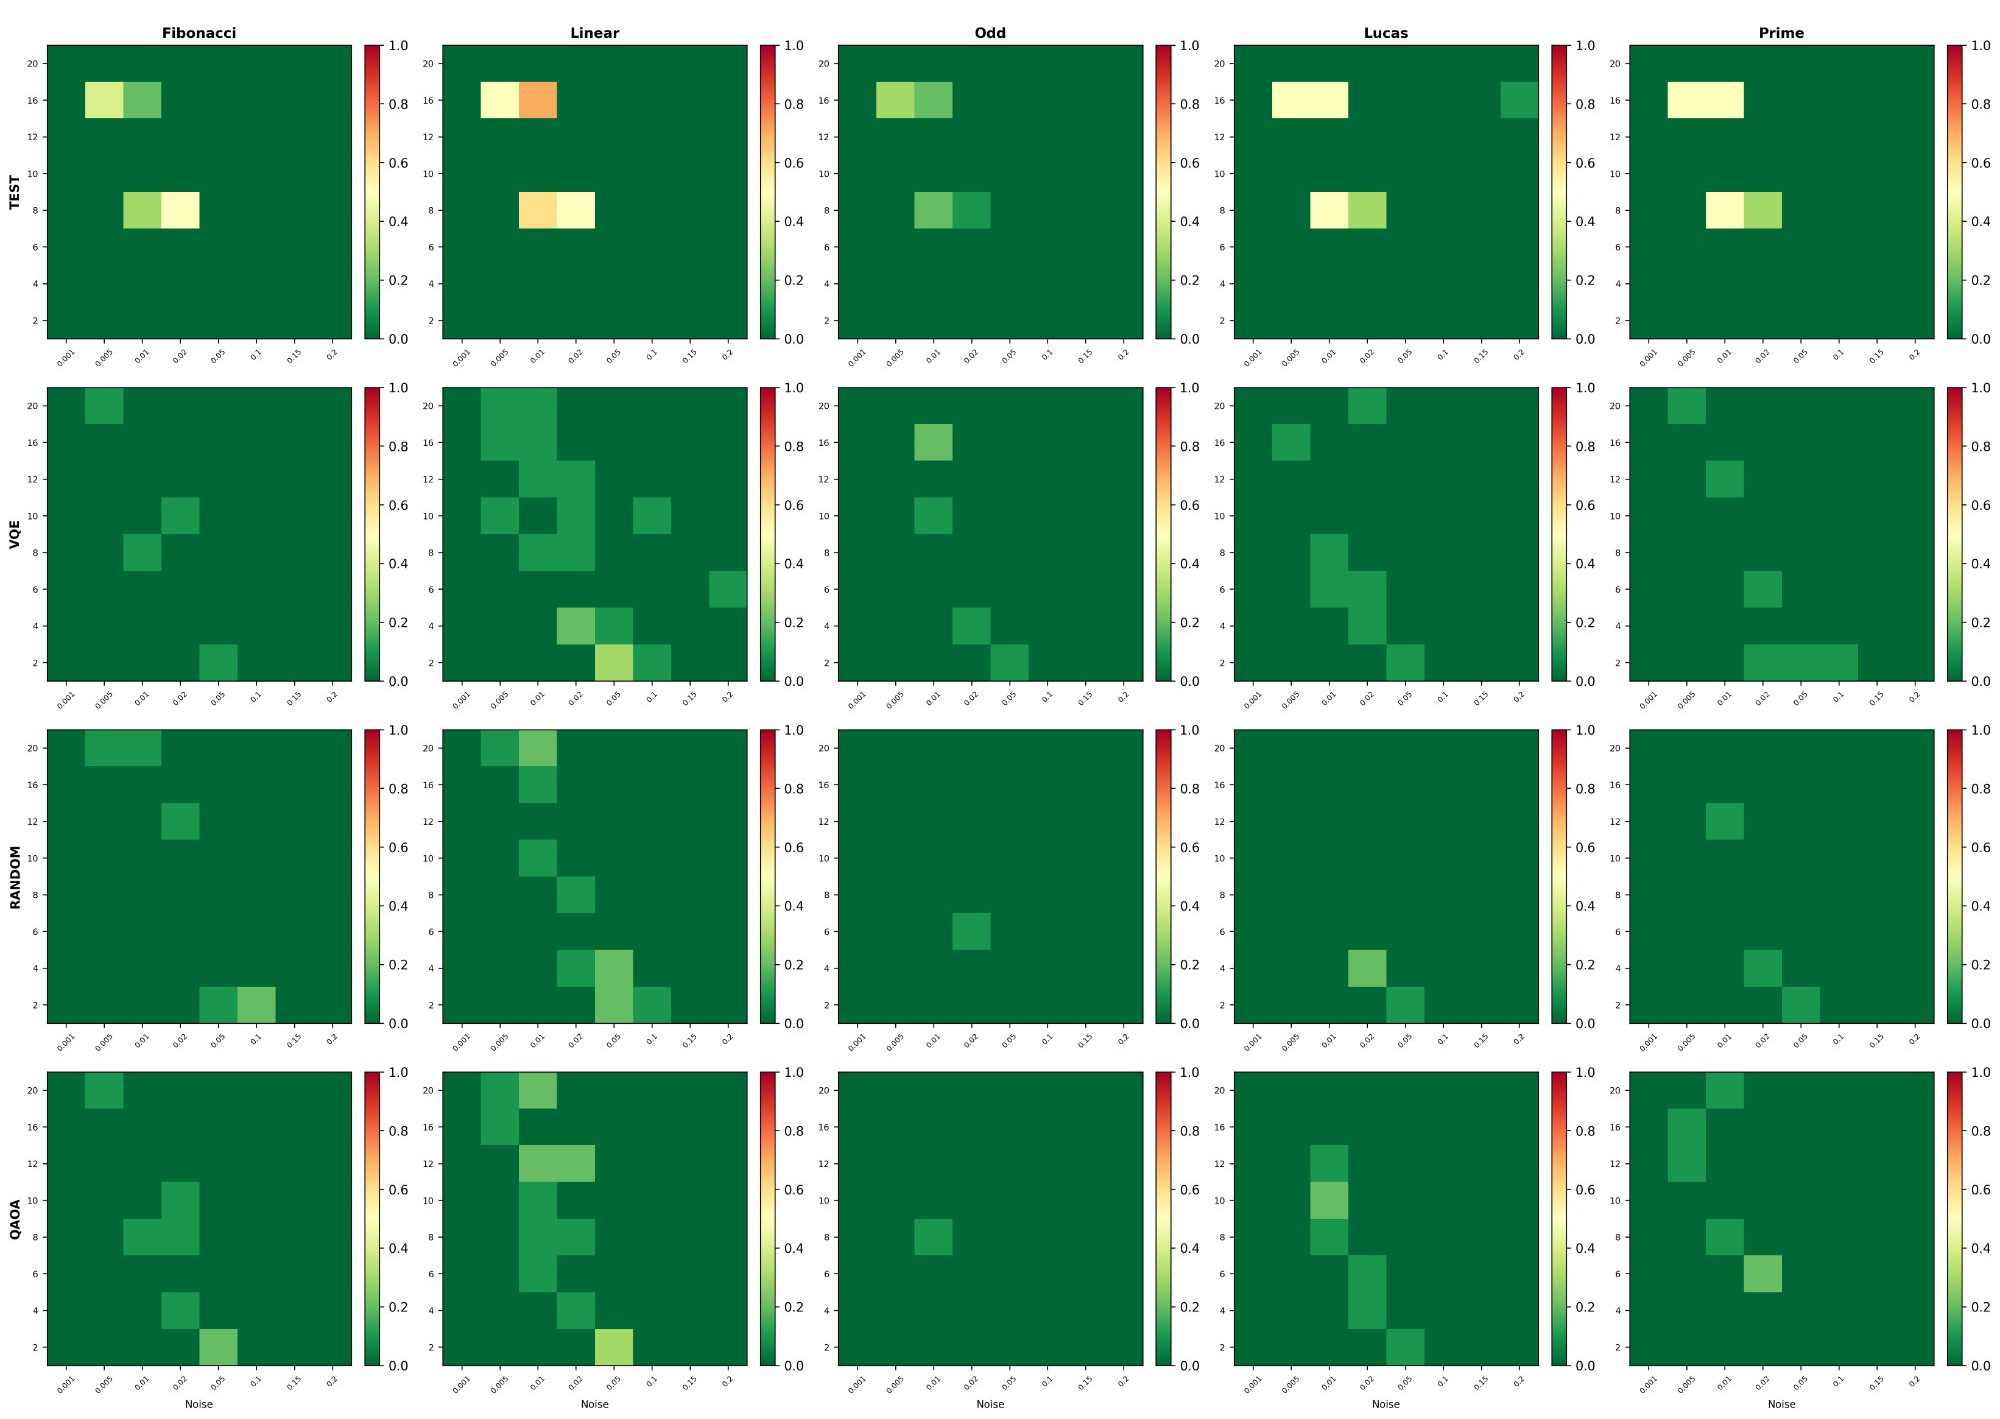
\includegraphics[width=\textwidth]{figC_v4_flag_rate_heatmaps.png}
  \caption{Stability filter flag rate across all circuit types (rows)
    and schedules (columns) at $n=2$, spanning depths
    $d\in\{2,4,6,8,10,12,16,20\}$ and noise levels
    $p\in\{0.001\text{--}0.2\}$.
    Green: 0\% flag rate (stable). Red: flagged.
    Flag rates are 0\% at $p\leq 0.01$, $d\leq 4$ across all
    circuit types and schedules.}
  \label{fig:heatmap}
\end{figure*}

\begin{figure*}[tp]
  \centering
  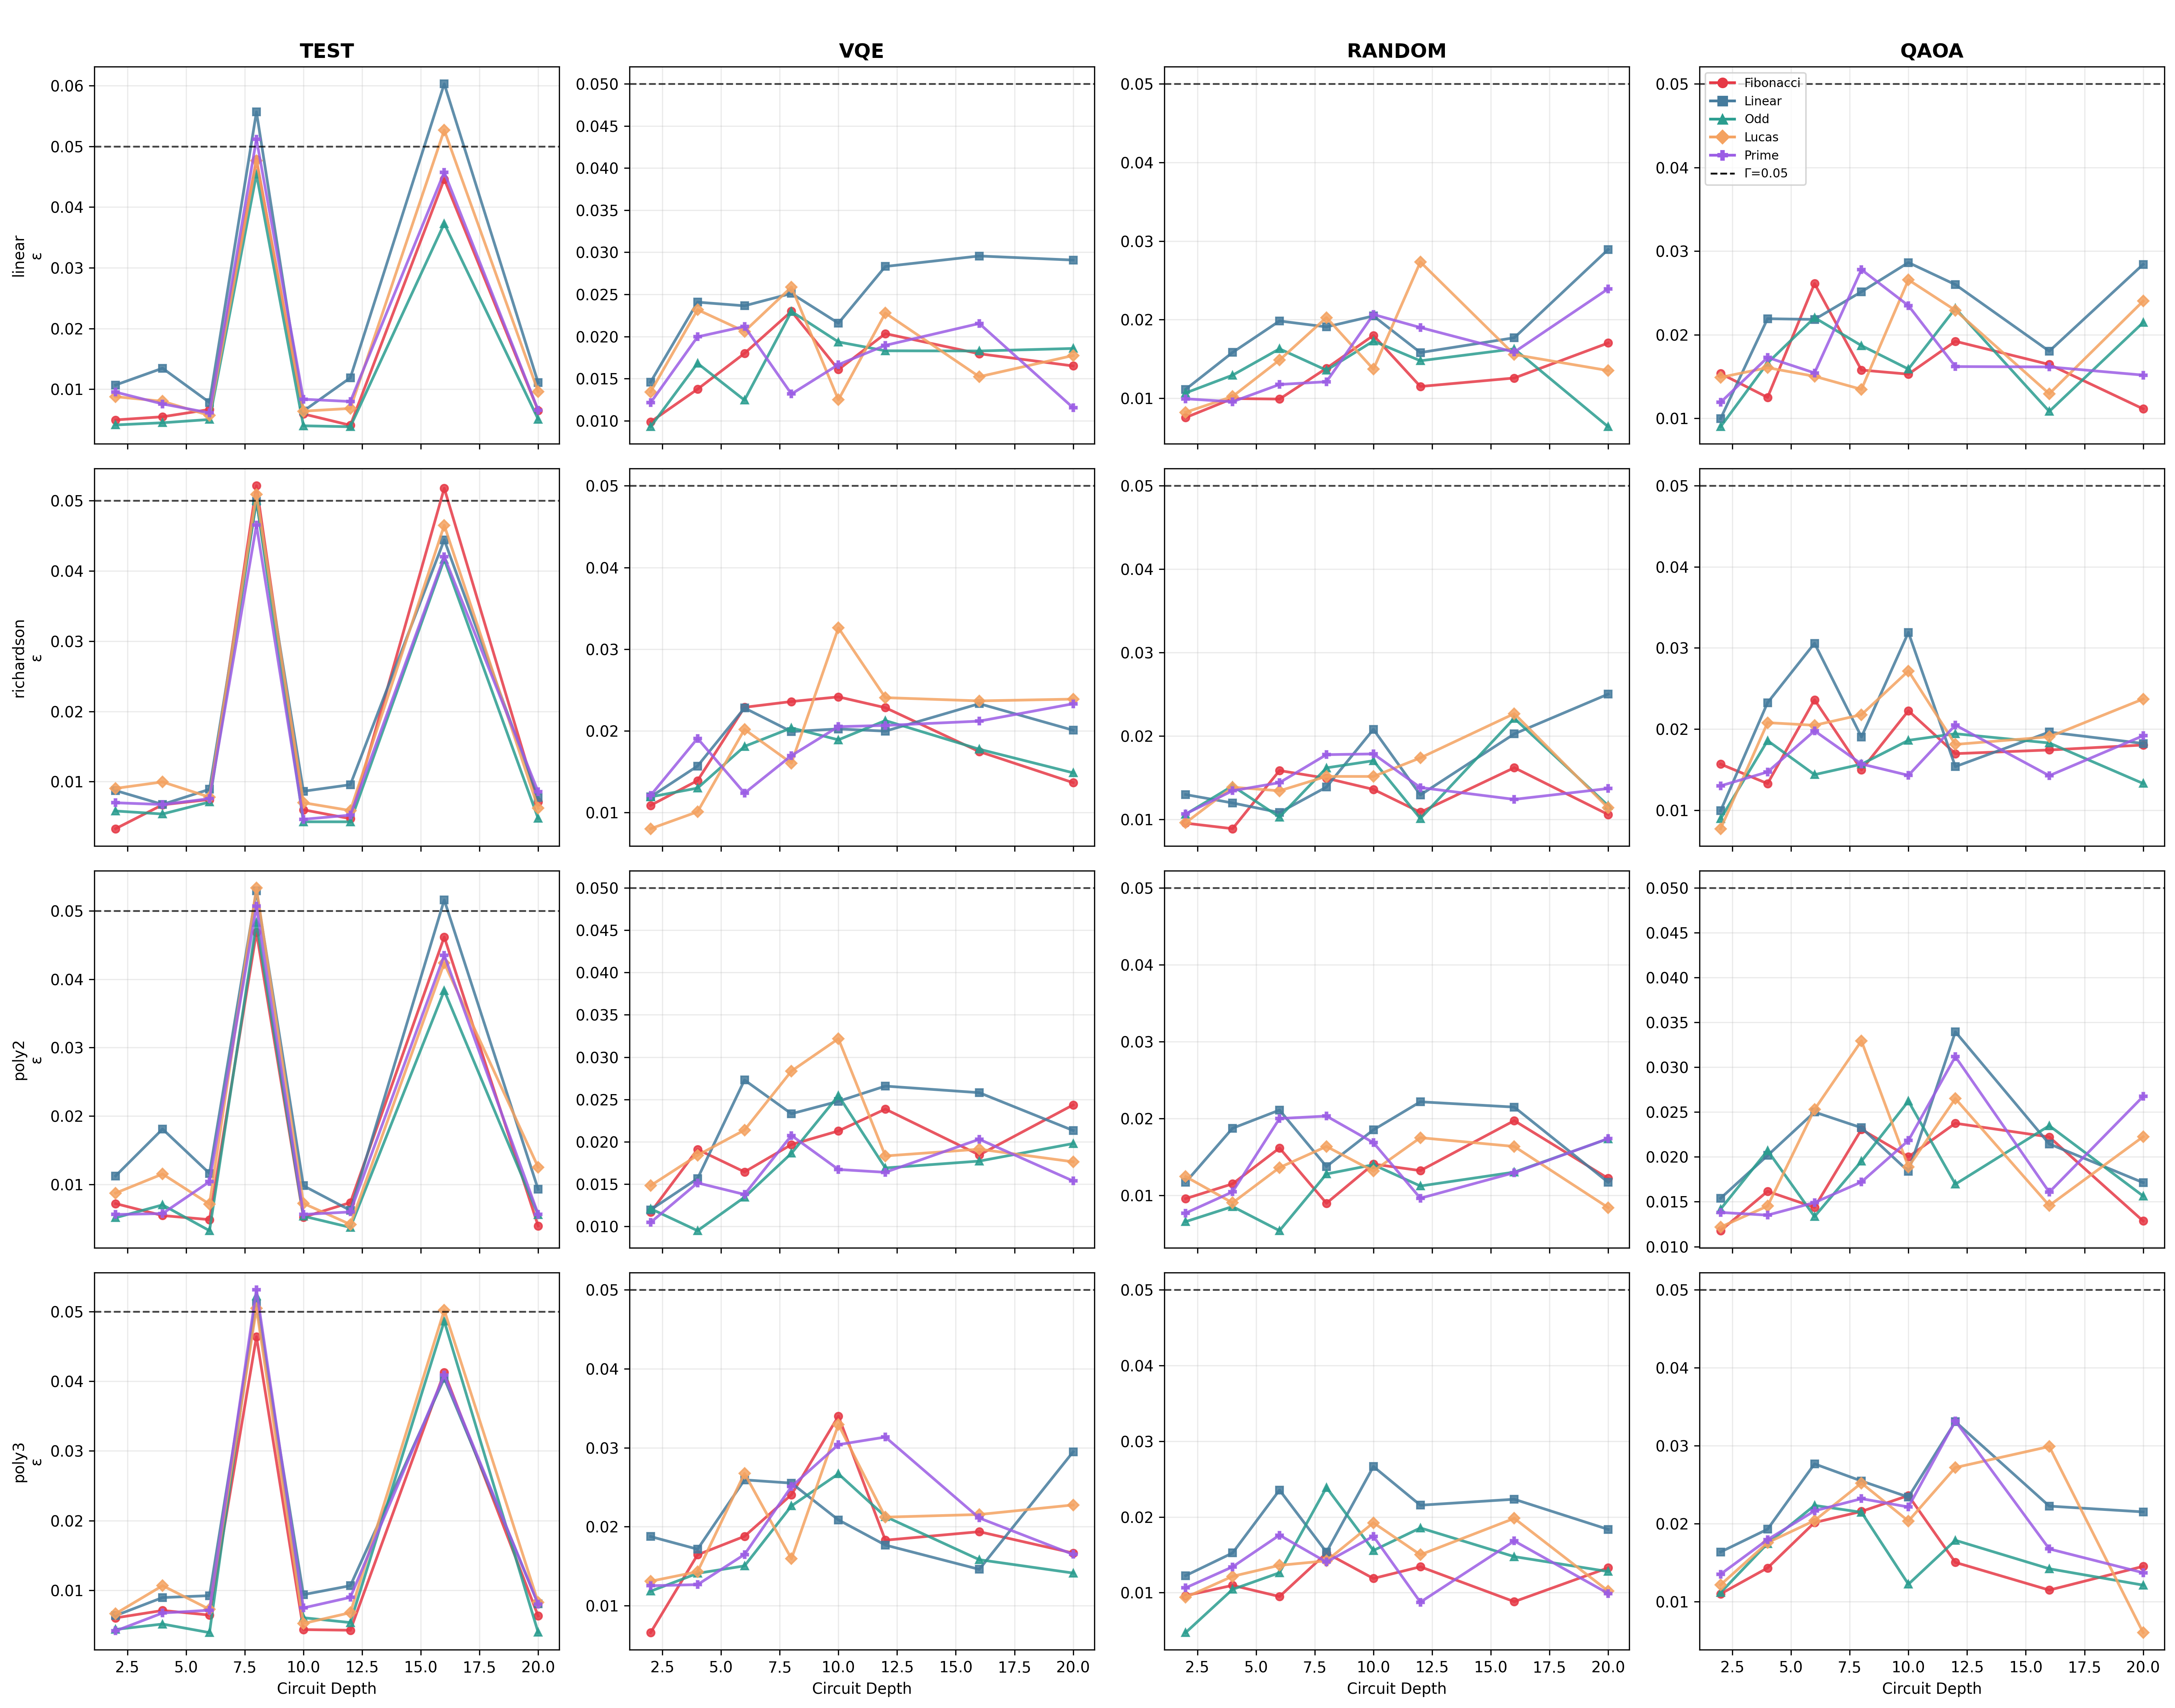
\includegraphics[width=\textwidth]{figE_v4_eps_vs_depth.png}
  \caption{$\varepsilon$ vs.\ circuit depth at $p=0.01$, $n=2$, for
    all five schedules (colours) across all four extrapolants (rows)
    and all circuit types (columns). All schedules remain below
    $\Gamma=0.05$ at $d\leq 4$. The test circuit exhibits sharp spikes
    at $d=8$ and $d=16$: the fixed $R_x(\pi/4)$ rotation drives
    $\langle Z_0 Z_1\rangle\to\pm 1$ at every eighth layer, maximising
    ZNE curve steepness. VQE, QAOA, and random circuits show no such
    periodicity. Dashed line: $\Gamma=0.05$.}
  \label{fig:eps_circuits}
\end{figure*}

\begin{figure*}[tp]
  \centering
  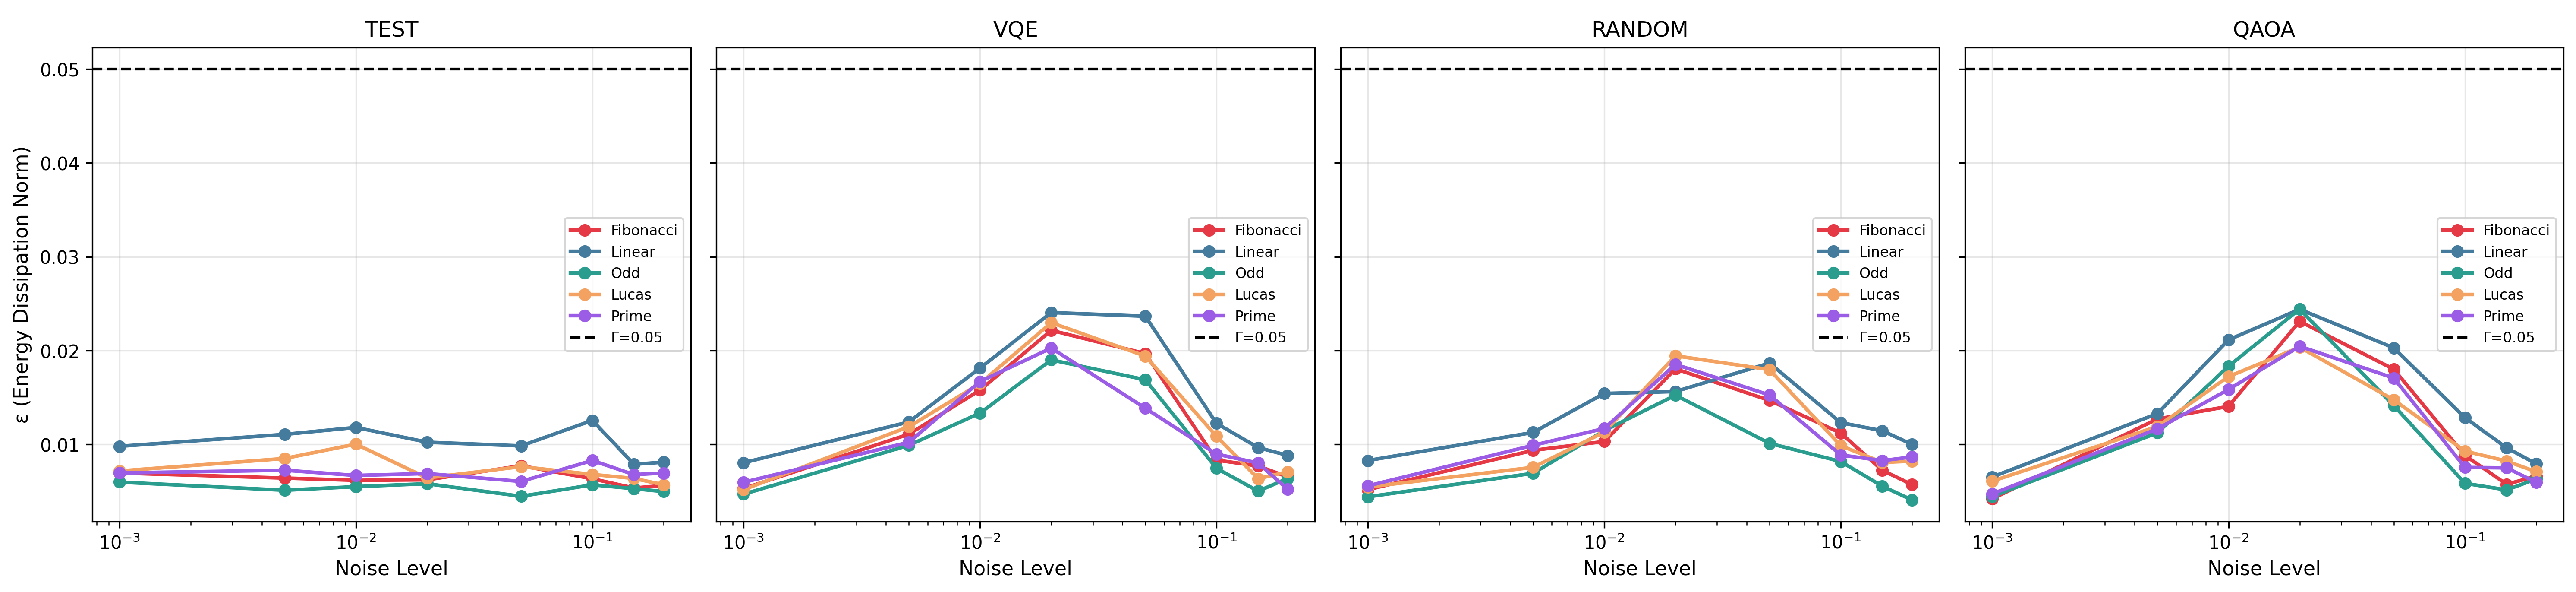
\includegraphics[width=\textwidth]{fig9_v4_schedule_comparison.png}
  \caption{Stability criterion $\varepsilon$ vs.\ noise level for all five
    schedules at $d=4$, $n=2$, linear extrapolant, across all four circuit
    types. Dashed line: $\Gamma=0.05$. Error bars: std over 10 trials,
    500 shots. All schedules remain well below $\Gamma$ at $p\leq 0.01$.}
  \label{fig:eps_schedules}
\end{figure*}
\subsection{Schedule Comparison Across Circuit Types}

All five schedules remain below $\Gamma=0.05$ at $p\leq 0.01$,
$d\leq 4$. The linear schedule produces the highest mean $\varepsilon$
at $n=2$ ($\bar\varepsilon=0.019$, averaged over four circuit types);
Fibonacci the lowest ($\bar\varepsilon=0.010$).
On VQE circuits, the linear schedule produces the highest $\varepsilon$
($\varepsilon=0.024$), likely because equal spacing at small scale
factors more uniformly samples the high-noise region of the
extrapolation curve. Fibonacci's coarser, golden-ratio-distributed
spacing produces lower $\varepsilon$ (0.014) despite reaching scale
factor~13. Lucas (mean $\bar\varepsilon=0.014$) and prime-anchored
(mean $\bar\varepsilon=0.014$) schedules perform comparably to each
other and sit between linear and Fibonacci across all circuits.
On random and QAOA circuits, all schedules converge to similar
$\varepsilon$ values, indicating the filter is schedule-agnostic for
unstructured circuits. The odd-integer schedule (mean
$\bar\varepsilon=0.013$) sits between Fibonacci and the Lucas/prime
group across all circuit types, consistent with its intermediate
spacing density. The Lucas schedule achieves the lowest ZNE
variance on random and QAOA circuits (Table~\ref{tab:extrapolants});
prime-anchored performs comparably to Fibonacci on test and random circuits.

\subsection{Qubit Scaling}

Table~\ref{tab:qubit} reports $\varepsilon$ at $d=4$, $p=0.01$ for
$n\in\{2,4,6\}$ (see also Fig.~\ref{fig:qubit_scaling}). In 19 of 20 circuit/schedule combinations,
$\varepsilon$ decreases monotonically with $n$: the decrease likely
reflects attenuation of correlations along longer noisy gate sequences,
smoothing the ZNE curve.
ZNE variance similarly decreases
($n=6$ std $\approx$ half of $n=2$).
The single non-monotone case (QAOA/linear: $n{=}4\ \varepsilon=0.00494$,
$n{=}6\ \varepsilon=0.00522$) represents a minor inversion well within
trial variance and does not affect the overall trend.

\begin{table}[H]
\caption{Energy norm $\varepsilon$ vs.\ qubit count ($d=4$, $p=0.01$,
  linear extrapolant). Monotone decrease in 19/20 cases;
  $^*$minor inversion within trial variance.}
\label{tab:qubit}
\centering\small
\setlength{\tabcolsep}{5pt}
\begin{tabular}{llccc}
\toprule
Circuit & Schedule  & $n{=}2$ & $n{=}4$ & $n{=}6$ \\
\midrule
Test & Fibonacci & 0.00545 & 0.00280 & 0.00132 \\
Test & Linear    & 0.01345 & 0.00275 & 0.00197 \\
Test & Odd       & 0.00447 & 0.00240 & 0.00064 \\
Test & Lucas     & 0.00801 & 0.00223 & 0.00121 \\
Test & Prime     & 0.00757 & 0.00141 & 0.00092 \\
\midrule
VQE  & Fibonacci & 0.01375 & 0.00738 & 0.00183 \\
VQE  & Linear    & 0.02408 & 0.00667 & 0.00247 \\
VQE  & Odd       & 0.01681 & 0.00543 & 0.00253 \\
VQE  & Lucas     & 0.02318 & 0.00701 & 0.00216 \\
VQE  & Prime     & 0.01996 & 0.00437 & 0.00191 \\
\midrule
Rand & Fibonacci & 0.00997 & 0.00298 & 0.00174 \\
Rand & Linear    & 0.01583 & 0.00440 & 0.00191 \\
Rand & Odd       & 0.01294 & 0.00375 & 0.00189 \\
Rand & Lucas     & 0.01023 & 0.00233 & 0.00223 \\
Rand & Prime     & 0.00956 & 0.00267 & 0.00240 \\
\midrule
QAOA & Fibonacci & 0.01249 & 0.00987 & 0.00410 \\
QAOA & Linear    & 0.02190 & 0.00494 & $0.00522^{*}$ \\
QAOA & Odd       & 0.01661 & 0.00590 & 0.00296 \\
QAOA & Lucas     & 0.01605 & 0.00799 & 0.00247 \\
QAOA & Prime     & 0.01727 & 0.00704 & 0.00182 \\
\bottomrule
\end{tabular}
\end{table}

\begin{figure*}[tp]
  \centering
  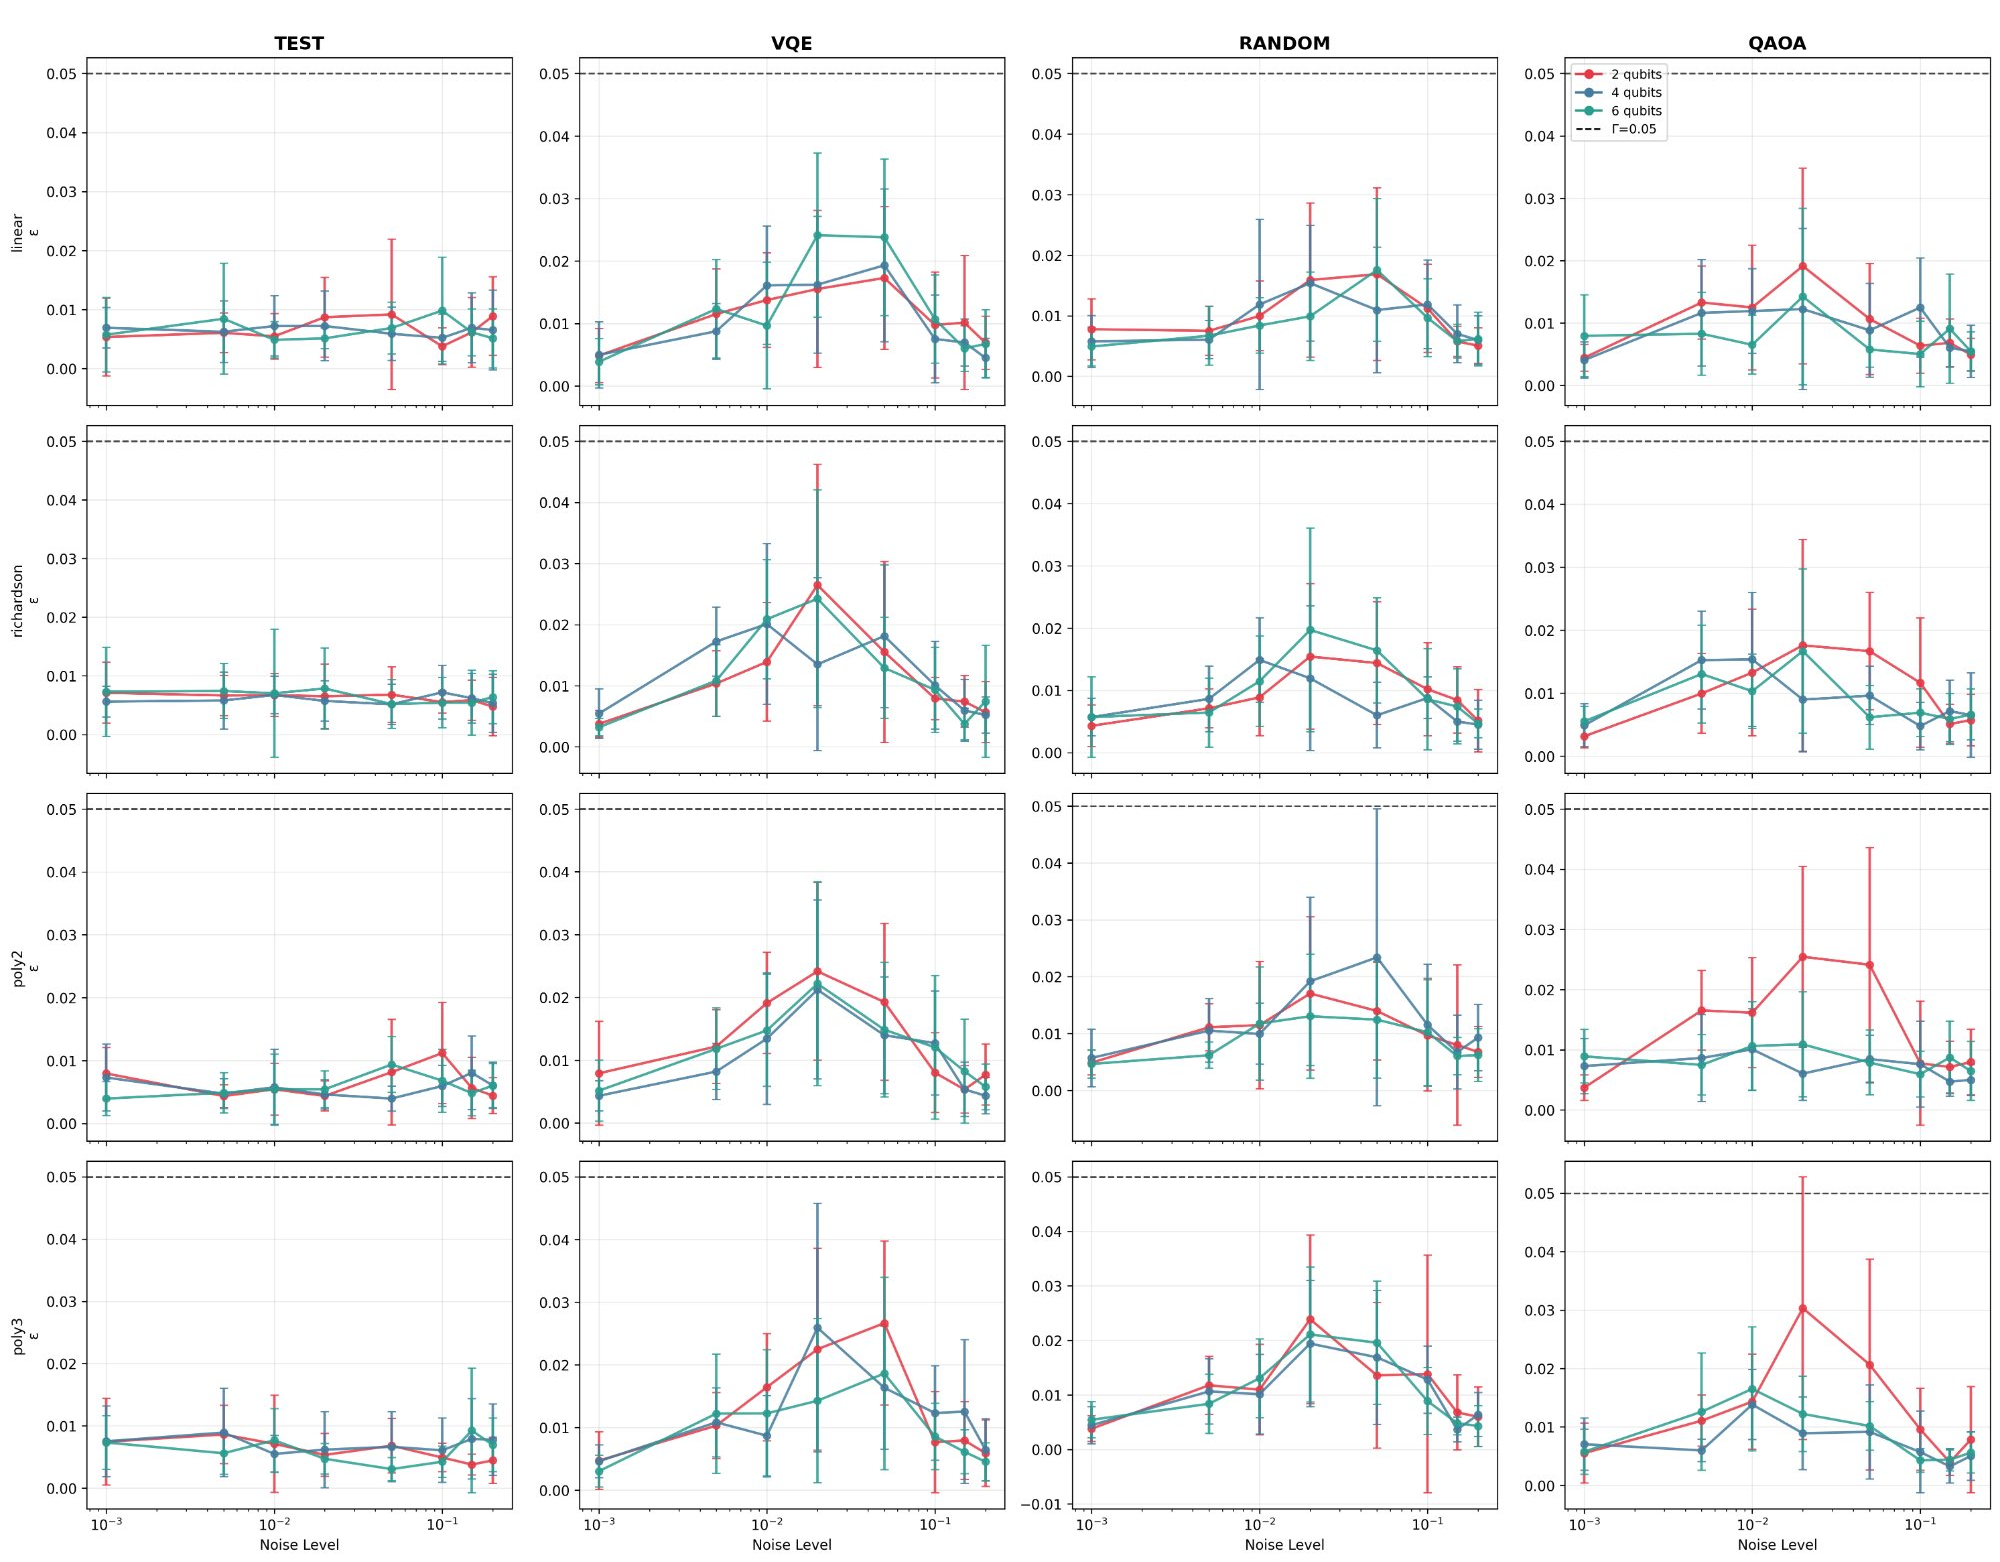
\includegraphics[width=0.97\textwidth]{figB_v4_eps_vs_noise_qubit_scaling.png}
  \caption{Energy norm $\varepsilon$ vs.\ noise level for
    $n\in\{2,4,6\}$ qubits, Fibonacci schedule, $d=4$,
    across all four circuit types and all four extrapolants (rows).
    $\varepsilon$ decreases monotonically with qubit count across
    nearly all combinations; minor inversions appear only in
    Richardson extrapolation, consistent with attenuation of
    correlations along longer noisy gate sequences.}
  \label{fig:qubit_scaling}
\end{figure*}

\subsection{Hardware Validation}
\label{sec:hardware}

We validated the stability filter on two IBM Quantum processors:
\textit{ibm\_fez} (Heron~r2, 156 qubits) and \textit{ibm\_torino}
(Heron~r1, 133~qubits), using global circuit folding with odd-integer
scale factors $\{1,3,5,9,13\}$ (Fibonacci-odd) and $\{1,3,5,7,9\}$
(linear-odd), $N=1024$ shots, and 5 trials per condition.
The hardware VQE circuit uses $R_y(\pi/4)$+CX in place of the
simulation's $R_y$+CZ ansatz; CX is the native two-qubit gate on both
devices and avoids the additional single-qubit overhead of
CZ~$=$~H$\cdot$CX$\cdot$H.
All 24 conditions across four circuit types
(test, VQE, random, QAOA), two schedules, and depths
$d\in\{2,4,6,8\}$ yield $\varepsilon<\Gamma_{\mathrm{sim}}=0.05$
(120 trials; 95\% C-P upper bound: $p_{\mathrm{flag}}<0.025$),
with a maximum observed $\varepsilon=0.00285$ --- $5.7\%$ of
$\Gamma_{\mathrm{sim}}$ (Table~\ref{tab:hardware}).

The Fibonacci schedule produces lower $\varepsilon$ than linear in all
four circuit types at $d=4$ (Fibonacci: $0.00047$--$0.00154$;
linear: $0.00120$--$0.00285$), consistent with the simulation finding.
ZNE output variance is substantially tighter on hardware
($\sigma_{\mathrm{ZNE}}=0.008$--$0.031$) than in simulation
($\sigma_{\mathrm{ZNE}}=0.022$--$0.594$), reflecting the lower
effective noise level of ibm\_fez and ibm\_torino
(equivalent to $p\approx0.001$ depolarizing,
versus the simulation reference of $p=0.01$).

At $d=8$, all ZNE outputs converge to $\langle O\rangle\approx -0.70$
regardless of circuit type or schedule, with $\varepsilon$ dropping
below $0.001$ --- lower than at $d=6$.
This reflects decoherence saturation in the heavily folded circuits
($\lambda=9,13$ producing up to 104 effective layers):
all scale-factor points cluster near the same value,
making the ZNE curve flat and hence $\varepsilon\approx 0$.
This reveals a boundary condition not present in simulation:
$\varepsilon$ measures curve \textit{smoothness} but cannot distinguish
reliable extrapolation from decoherence-induced saturation.
The filter correctly produces low $\varepsilon$ in both cases;
a complementary check (e.g.\ comparing $\langle O\rangle_{\lambda=1}$
against the saturated value) would disambiguate the two regimes.
This is consistent with the Limitations noted in Section~\ref{sec:discussion}.

\begin{table}[H]
\caption{Hardware validation: $\varepsilon$ on ibm\_fez and ibm\_torino.
  $N=1024$ shots, 5 trials, odd-only scale factors $K=5$.
  All 24 conditions pass $\Gamma_{\mathrm{sim}}=0.05$ and
  $\Gamma_{\mathrm{hw}}=0.10$.
  Fibonacci $<$ Linear in all 4 circuit types at $d=4$.}
\label{tab:hardware}
\centering\small
\setlength{\tabcolsep}{4pt}
\begin{tabular}{llcrcc}
\toprule
Circuit & Schedule & $d$ & $\varepsilon$ (mean$\pm$std) & ZNE & Device \\
\midrule
Test    & Fibonacci & 2 & $0.00188\pm0.00138$ & $-0.295$ & ibm\_fez \\
Test    & Fibonacci & 4 & $0.00154\pm0.00134$ & $+0.109$ & ibm\_fez \\
Test    & Fibonacci & 6 & $0.00207\pm0.00091$ & $+0.024$ & ibm\_torino \\
Test    & Fibonacci & 8 & $0.00057\pm0.00032$ & $-0.704$ & ibm\_torino \\
Test    & Linear    & 2 & $0.00188\pm0.00119$ & $-0.295$ & ibm\_fez \\
Test    & Linear    & 4 & $0.00285\pm0.00276$ & $+0.086$ & ibm\_fez \\
Test    & Linear    & 6 & $0.00279\pm0.00196$ & $+0.005$ & ibm\_torino \\
Test    & Linear    & 8 & $0.00053\pm0.00040$ & $-0.709$ & ibm\_torino \\
\midrule
VQE     & Fibonacci & 2 & $0.00179\pm0.00160$ & $-0.193$ & ibm\_fez \\
VQE     & Fibonacci & 4 & $0.00047\pm0.00032$ & $-0.548$ & ibm\_fez \\
VQE     & Fibonacci & 6 & $0.00133\pm0.00138$ & $-0.345$ & ibm\_torino \\
VQE     & Fibonacci & 8 & $0.00045\pm0.00010$ & $-0.706$ & ibm\_torino \\
VQE     & Linear    & 2 & $0.00098\pm0.00038$ & $-0.183$ & ibm\_fez \\
VQE     & Linear    & 4 & $0.00120\pm0.00049$ & $-0.550$ & ibm\_fez \\
VQE     & Linear    & 6 & $0.00202\pm0.00127$ & $-0.352$ & ibm\_torino \\
VQE     & Linear    & 8 & $0.00125\pm0.00087$ & $-0.707$ & ibm\_torino \\
\midrule
Random  & Fibonacci & 2 & $0.00084\pm0.00064$ & $-0.785$ & ibm\_fez \\
Random  & Fibonacci & 4 & $0.00073\pm0.00052$ & $-0.562$ & ibm\_fez \\
Random  & Linear    & 2 & $0.00106\pm0.00096$ & $-0.779$ & ibm\_fez \\
Random  & Linear    & 4 & $0.00259\pm0.00224$ & $-0.572$ & ibm\_fez \\
\midrule
QAOA    & Fibonacci & 2 & $0.00162\pm0.00077$ & $+0.048$ & ibm\_fez \\
QAOA    & Fibonacci & 4 & $0.00112\pm0.00044$ & $+0.497$ & ibm\_fez \\
QAOA    & Linear    & 2 & $0.00129\pm0.00108$ & $+0.034$ & ibm\_fez \\
QAOA    & Linear    & 4 & $0.00178\pm0.00101$ & $+0.503$ & ibm\_fez \\
\bottomrule
\end{tabular}
\end{table}

\subsection{Hessian Analysis}

No singular regions ($\det H\approx 0$) were detected at $p\leq 0.01$
for any depth or qubit count, consistent with stability filter results.
At $p\geq 0.1$, $d\geq 12$, singular regions appear for all four
circuit types. Singularity density increases monotonically with both
depth and noise through $d=20$. This co-emergence of Hessian
singularities with $\varepsilon\geq\Gamma$ flags provides qualitative
corroboration that both diagnostics identify the same physically
unstable regime.

% ============================================================
\clearpage  % flush Results floats before Discussion
\section{Discussion}
\label{sec:discussion}
% ============================================================

The stability filter provides an $\mathcal{O}(K)$ arithmetic
post-hoc reliability check --- $K$ multiply-accumulate operations
on the expectation values already collected for extrapolation.
Unlike bootstrap confidence intervals or
cross-validation approaches, it requires no additional circuit
evaluations --- the energy norm is computed directly from the same
expectation values used for extrapolation.

The Fibonacci schedule's golden-ratio spacing means that consecutive
Fibonacci numbers are coprime ($\gcd(F_n, F_{n+1})=1$, provable by
the Euclidean algorithm), so no two consecutive scale factors share
a common factor greater than 1. This may reduce systematic correlations
in the noise amplification. The Lucas and prime-anchored schedules share
this non-harmonic spacing property and produce comparable $\varepsilon$
values ($\bar\varepsilon\approx 0.014$ for both), suggesting the benefit
derives from non-uniform spacing generally rather than the Fibonacci
recurrence specifically. A rigorous theoretical justification is left
for future work.

The qubit-scaling result ($\varepsilon$ decreasing with circuit width)
likely reflects attenuation of correlations along longer noisy gate
sequences, smoothing the $\langle Z_0 Z_1\rangle$ extrapolation curve.
The filter is therefore most conservative at $n=2$ and progressively
more permissive at larger qubit counts --- a desirable property for
deployment.

For practical schedule and extrapolant selection: Fibonacci minimises
$\varepsilon$ (lowest energy norm, best filter stability); Lucas
minimises ZNE output variance on unstructured circuits (random, QAOA);
linear and odd-integer remain valid baselines with well-understood
behaviour. Across all five schedules, linear extrapolation produces
the lowest and most consistent ZNE variance and is the recommended
extrapolant for reliability-focused deployment.

\textit{Limitations.} The threshold $\Gamma$ requires calibration per
noise regime. The flag-rate claim applies at $d\leq 4$; at greater
depths accumulated gate noise triggers flagging, which is physically
correct. Extension to higher-degree extrapolants, adaptive methods,
and problem-specific circuits remains future work.

All results are obtained via density matrix simulation assuming a
single-qubit depolarising noise model applied independently after
every gate. Real hardware exhibits correlated errors, crosstalk, and
non-Markovian noise that may shift absolute $\varepsilon$ values and
require threshold recalibration. However, the qualitative behaviour
--- filter discrimination at low noise, circuit-type hierarchy, and
monotone qubit scaling --- is expected to be robust to moderate noise
model mis-specification, as the filter depends on the \textit{shape}
of the ZNE curve rather than the specific noise mechanism.
Hardware validation on ibm\_fez and ibm\_torino
(Section~\ref{sec:hardware}) confirms zero flags across 24 conditions
on real devices; robustness under amplitude-damping and correlated
noise models remains an important direction for future work.

% ============================================================
\section{Conclusion}
% ============================================================

We introduced a fluid-dynamic stability filter and a family of five
noise scaling schedules (Fibonacci, Lucas, prime-anchored, linear, odd)
for ZNE, implemented in open-source Python (Cirq, Mitiq).
Results across 153,600 runs confirm three principal findings:

\begin{enumerate}\setlength{\itemsep}{1pt}
  \item Zero flags in 14,400 trials at $p\leq 0.01$, $d\leq 4$
    (95\% C-P upper bound: $p_{\mathrm{flag}}<0.00022$).
  \item Circuit-type $\varepsilon$ hierarchy:
    VQE $>$ QAOA $>$ random $>$ test --- a previously uncharacterised
    dependence, now extended to QAOA and three qubit counts.
  \item $\varepsilon$ decreases monotonically with qubit count in
    19/20 cases; ZNE variance similarly decreases.
  \item Hardware validation on ibm\_fez and ibm\_torino: zero flags
    in 120 trials (24 conditions $\times$ 5 trials) across all four
    circuit types, $d\in\{2,4,6,8\}$; maximum $\varepsilon=0.00285$
    ($5.7\%$ of $\Gamma$); Fibonacci $<$ Linear in all four circuit
    types at $d=4$.
\end{enumerate}

Linear extrapolation produces the lowest and most consistent variance
across all configurations and all five schedules ($\sigma=0.324$--$0.594$
vs.\ Richardson/poly3 which reach $\sigma>0.6$ on some schedule/circuit
combinations); Lucas achieves the lowest variance on random and QAOA
circuits and is recommended for those use cases.
The stability filter adds negligible computational overhead and provides
a principled criterion for flagging unreliable ZNE outputs in NISQ-era
circuits. Code and data are available at:
\href{https://github.com/OfficialChaos/Quantum-Vortex-QEM}{\texttt{github.com/OfficialChaos/Quantum-Vortex-QEM}}
(Zenodo DOI:~10.5281/zenodo.18827720).

% ============================================================
\section*{Acknowledgments}
% ============================================================

The author thanks the developers of Cirq and Mitiq for their
open-source quantum computing tools. Simulations were conducted on
a personal workstation. Hardware experiments were conducted using
IBM Quantum services; ibm\_fez and ibm\_torino are devices of the
IBM Quantum Network. No external funding to declare.

% ============================================================
\clearpage   % flush all pending floats (Fig.4, Fig.5, Table 3) before references
\begin{thebibliography}{18}
\bibitem{Preskill2018}
  J.~Preskill, ``Quantum computing in the NISQ era and beyond,''
  Quantum \textbf{2}, 79 (2018).
\bibitem{Temme2017}
  K.~Temme, S.~Bravyi, and J.~M.~Gambetta,
  ``Error mitigation for short-depth quantum circuits,''
  Phys.\ Rev.\ Lett.\ \textbf{119}, 180509 (2017).
\bibitem{Endo2018}
  S.~Endo, S.~C.~Benjamin, and Y.~Li,
  ``Practical quantum error mitigation for near-future applications,''
  Phys.\ Rev.\ X \textbf{8}, 031027 (2018).
\bibitem{Li2017}
  Y.~Li and S.~C.~Benjamin,
  ``Efficient variational quantum simulator incorporating active error
  minimization,''
  Phys.\ Rev.\ X \textbf{7}, 021050 (2017).
\bibitem{LaRose2022}
  R.~LaRose \textit{et~al.},
  ``Mitiq: A software package for error mitigation on noisy quantum
  computers,'' Quantum \textbf{6}, 774 (2022).
\bibitem{Viola1998}
  L.~Viola and S.~Lloyd,
  ``Dynamical decoupling of open quantum systems,''
  Phys.\ Rev.\ Lett.\ \textbf{81}, 2594 (1998).
\bibitem{GiurgicaTiron2020}
  T.~Giurgica-Tiron, Y.~Hindy, R.~LaRose, A.~Mari, and W.~J.~Zeng,
  ``Digital zero noise extrapolation for quantum error mitigation,''
  in \textit{Proc.\ IEEE Int.\ Conf.\ Quantum Comput.\ Eng.}
  (2020) pp.\ 306--316.
\bibitem{Krebsbach2022}
  M.~Krebsbach, B.~Trauzettel, and A.~Calzona,
  ``Optimization of Richardson extrapolation for quantum error mitigation,''
  Phys.\ Rev.\ A \textbf{106}, 062436 (2022).
\bibitem{Mohammadipour2025}
  P.~Mohammadipour and X.~Li,
  ``Direct analysis of zero-noise extrapolation: Polynomial methods,
  error bounds, and simultaneous physical-algorithmic error mitigation,''
  Quantum \textbf{9}, 1909 (2025).
\bibitem{Hour2024}
  L.~Hour, M.~Go, and Y.~Han,
  ``Improving zero-noise extrapolation for quantum-gate error mitigation
  using a noise-aware folding method,'' arXiv:2401.12495 (2024).
\bibitem{Zhang2025}
  A.~Zhang \textit{et~al.},
  ``Demonstrating quantum error mitigation on logical qubits,''
  Nat.\ Commun.\ \href{https://doi.org/10.1038/s41467-025-67768-4}%
  {10.1038/s41467-025-67768-4} (2025).
\bibitem{Sohn2025}
  H.~Sohn \textit{et~al.},
  ``Application of zero-noise-extrapolation-based quantum error mitigation
  to a silicon spin qubit,''
  Phys.\ Rev.\ A \textbf{112}, 012408 (2025).
\bibitem{Raymond2025}
  J.~Raymond \textit{et~al.},
  ``Quantum error mitigation in quantum annealing,''
  npj Quantum Inf.\ \href{https://doi.org/10.1038/s41534-025-00977-3}%
  {10.1038/s41534-025-00977-3} (2025).
\bibitem{Raissi2019}
  M.~Raissi, P.~Perdikaris, and G.~E.~Karniadakis,
  ``Physics-informed neural networks: A deep learning framework for
  solving forward and inverse problems involving nonlinear PDEs,''
  J.\ Comput.\ Phys.\ \textbf{378}, 686 (2019).
\bibitem{Google2023}
  Google Quantum AI,
  ``Suppressing quantum errors by scaling a surface code logical qubit,''
  Nature \textbf{614}, 676 (2023).
\bibitem{Tao2016}
  T.~Tao,
  ``Finite time blowup for an averaged three-dimensional
  Navier-Stokes equation,''
  J.\ Amer.\ Math.\ Soc.\ \textbf{29}, 601 (2016).
\bibitem{Wang2025}
  Y.~Wang \textit{et~al.},
  ``Discovery of unstable singularities,''
  arXiv:2509.14185 [math.AP] (2025).
\bibitem{Cirq2023}
  Cirq Developers,
  ``Cirq: A Python framework for creating, editing, and invoking NISQ
  circuits,'' \url{https://quantumai.google/cirq} (2023).
\end{thebibliography}

\end{document}
